%%%%%%%%%%%%%%%%%%%%%%%%%%%%%%%%%%%%%%%%%%%%%%%%%%%%%%%%%%%%%%%%%%%%%%
%
%  Humanoids 2005
%

\documentclass[conference]{./sty/IEEEtran}

%  usepackage goes here.
\usepackage{cite}
\usepackage{graphicx}
\graphicspath{{./figures/}}

\begin{document}

\title{Exploring the world through grasping: Hitoshi's revenge}

\author{\authorblockN{Lorenzo Natale, Francesco Orabona, Fabio Berton, Giorgio Metta, Giulio Sandini}
\authorblockA{LIRA-Lab, DIST\\University of Genoa\\
Viale Causa 13, 16145, Genoa, Italy\\
Email: \{nat, bremen, fberton, pasa, sandini\}@liralab.it}}

\maketitle

\begin{abstract}

\iflong
\begin{abstract}
\else
\begin{Abstract}
\fi
 
Vision and manipulation are inextricably intertwined in the primate
brain.  Tantalizing results from neuroscience are illuminating the
mixed representations used by the brain in reaching, grasping, and
object recognition.  We wish to instantiate these results in robotic
form to probe their technical advantages and verify that the
associated models are at least consistent and without lacunae.

We believe it would be missing the point to investigate this on a
platform where dextrous manipulation and sophisticated machine vision
are already implemented (if such a platform existed).

In this paper, we show how we can take a simple precursor to manipulation,
namely poking and prodding, and already realize significant advantages in
visual processing, and make enough progress to develop a system that
is functionally analogous to models coming out of neuroscience.

We show how operational concepts can actually lead to well grounded
objects.


\ifverbose
For the purposes of manipulation, we would like to know what parts of
the environment are physically coherent ensembles -- that is, which
parts will move together, and which are more or less independent.  It
takes a great deal of experience before this judgement can be made
from purely visual information.  This paper develops active strategies
for acquiring that experience through experimental manipulation, using
tight correlations between arm motion and optic flow to detect both
the arm itself and the boundaries of objects with which it comes into
contact.  We argue that following causal chains of events out from
the robot's body into the environment allows for a very natural
developmental progression of visual competence, and relate this idea 
to results in neuroscience.
\fi

\ifverbose
For the purpose of understanding development we would like to present
causality as a possible principle to frame a number of neural science
results coherently. We will show how this can lead also to an
implementation in an artificial system following the epigenetic
approach. To this purpose we will show different levels of causal
linkages, or instances of the general principle, which allow tasks of
increasing complexity to be implemented.  Action and the physical
interaction of the robot with the environment play a fundamental role.
In an ecological perspective, the role of this physical interaction
for developing categorization and object undestanding is emphasized.
\fi

%%{\bf \em
%%\iflong
%%(long version)
%%\else
%%(short version)
%%\fi
%%}

\iflong
\end{abstract}
\else
\end{Abstract}
\fi

\end{abstract}


\section{Outline}

The sad fate of most robot software

Modularity in robotics

YARP: Yet Another Robot Platform

Excising communication ``plumbing'' from code

Excising device dependencies from code

Conclusions


\section{Sad fate}

Many robot projects are ``black holes'', in terms of software.  A lot
of software gets sucked in, but very little comes out.  Once a piece
of software has been adapted to a particular robot, it takes a lot
of work to extricate it again and apply it to another.

Obviously the answer to this problem is modularity.  So there are 
now many architectures/frameworks/... for modular robot systems.
The prime concern for any such system should be that it is not
a ``black hole'' -- that once a piece of software has been adapted
to a particular framework, it takes a lot of work to extricate it
again and apply it to another.  That would be a bit self-defeating.

We study YARP from this perspective.  How sticky is resultant user
code to the robot and to the framework itself?


\section{Free and Open Source}

Useful, more malleable.

Has the pragmatic benefit that a user of the software can
modify and integrate it to their hearts content without the 
pain of dealing with opaque binaries.

Has the revolutionary benefit that the user is not trapped in the role
of being a ``consumer'' of software, but can also be a publisher of
the changes, additions, and integrative work they do in an effective
form.  This is achieved by explicitly granting far more rights to
users than they have under the law of most countries, contrasting with
agreeably with the formerly more common practice of attempting to
minimize user rights.  These rights are typically granted
conditionally; a user may only make use of these extended rights if
(for example) distributed code is always available in its most useful
original (source) form, with compatible freedoms attached to it.  This
condition seeks to balance freedoms of individuals versus benefit to
the group.  The freedom to distribute code in obscure (compiled) forms



Split between people who emphasize pragmatic concerns and those
who emphasize freedom.  Just cite the issue, no need to revisit
it here.


\section{CMake}

Open-source, deals well with various IDEs and command-line development.

Not as familiar as autoconf/automake/... etc.

Has the excellent property of being simpler than making Makefiles
or configuring a project, when external libraries are involved.

The big downside is that the language is unfamiliar and a bit ugly.
It is simple and well-documented, but quirky.  An alternative with
some similar properties, scons, uses python instead.  The ant system
uses with java also seems cleaner.  However, it gets the job
done, and has the huge advantage of not being dependent on an
external language being installed.

CMake is free and open-source, with a healthy community of 
developers.



\section{Call for publication}

As a research community, we both read and produce papers, building on
each others' work.

We also both acquire and produce software

Our software tends to die with our projects

Sad!  Software collaboration speeds things up

Research groups that all use a specific robot (Khepera, Pioneer, AIBO,
...) often form a natural software community

But each alone is a small subset of robotics

Groups developing new robots face obstacles

Differences in sensors, actuators, bodies...

Differences in processors, operating systems, libraries, frameworks,
languages, compilers...

Big barriers to software collaboration


\section{Modularity}

Constant hardware flux

Parts change rapidly

Interfaces change slowly

Lots of software grew and evolved alongside the changing hardware

Parts change rapidly

Interfaces change slowly

``Modularity'' is rewarded


\subsection{Broom}

The way parts interact can last longer than the parts themselves

E.g. an eternal broom

replace broom head

replace broom handle


\subsection{Theseus}

Long-lived software is like the Ship of Theseus

The mast gets replaced

The planks get replaced

Over time, everything may get replaced

In philosophy, this is a ``paradox of identity''

For us, it's just our job


\subsection{dark path}

The opposite of a modular system is a coupled one.

In a ``coupled'' system, changes in one part trigger changes in another.

Coupling leads to complexity

Complexity leads to confusion

Confusion leads to suffering

This is the path to the Dark Side

\subsection{modular robots}

Robot software is notoriously hardware-specific and task-specific

Both hardware and target tasks change quickly, even within the
lifetime of one project

Our humanoid robots are far more complex than one person can build and
maintain, both in terms of hardware and software

They need to be modular


\subsection{YARP}

YARP is an open-source software library  for humanoid robotics

History

An MIT / LIRA-Lab collaboration

Born on Kismet, grew on COG

With a major overhaul, now used by RobotCub consortium

Exists as an independent open source project

C++ source code


\subsection{Things we use}

CMake slide.

SWIG slide.


\subsection{What is YARP for}


Factor out details of data flow between programs from program source code

Data flow is very specific to robot platform, experimental setup,
network layout, communication protocol, etc.

Useful to keep ``algorithm'' and ``plumbing'' separate

Factor out details of devices used by programs from program source code

The devices can then be replaced over time by comparable alternatives;
code can be used in other systems


\section{Literature}

The literature of a research community both expresses its ideas, and
aids in their evolution

Published ideas are read, evaluated, and built upon

Useful advances get published

Publication of software can speed progress

Facilitates evaluating and comparing approaches

Brings new research topics into reach

Publish or perish!



\subsection{A subsection ?}
just in case we need a subsection.
\section{The robotic platform}
\label{sect:robot}

\begin{figure}
\centering
\includegraphics[width=3in]{robot1}
\caption{The robotic platform: The Babybot.}
\label{fig-platform}
\end{figure}

The experiments reported in this paper were performed by using an upper torso humanoid robot called Babybot (Figure~\ref{fig-platform}). The Babybot consists of a head, an arm and a hand. The head has five degrees of freedom, and it is equipped with two cameras, two microphones and a set of gyroscopes. The cameras can pan independently and tilt around a common axis; the remaining degrees of freedom allows the head to pan and tilt at the level of the neck. The arm is an industrial PUMA 260 manipulator. The hand is mounted on the arm end point. It consists of a total of 16 degrees of freedom actuated by only 6 motors. Its five fingers are thus largely underactuated: the thumb and index are controlled independently by two motors each, whereas the remaining two motors are connected to the middle, ring and small finger which form a single virtual joint. The coupling between each joint and the motors is achieved by means of springs which give the hand a certain degree of compliance and elasticity. Magnetic potentiometers provide position and force feedback at each joint whereas force sensing resistors on the palm and fingers provide tactile feedback (see figure~\ref{fig-platform} and figure~\ref{fig-platform2}). A more detailed description of the hand can be found in \cite{natale04thesis}.

\begin{figure}
\centering
\includegraphics[width=3in]{robot2}
\caption{Details of the hand of the Babybot.}
\label{fig-platform2}
\end{figure}


\section{Visual System}
To have a wide field of view and a small image size we use log-polar images \cite{sandini80retinalike}. They mimic the photoreceptors distribution in the retina and the topological trasform from the retina to the visual cortex. In these images we have only a small center area with a high resolution (fovea) while in the periphery the resolution decrease exponentially moving away from the center. Like in humans, there is the need to move the sensor to take high resolution snapshots of important points in the scene, according to a given task or simple to quickly gather information about the scene. That is there is the need to have a system to select information points and to deeply analyze them.

To precisely manipulate an object the robot must be able to segment a scene in objects, in particular to segment an object from its background. It is not enough to poorly localize the object, we need a segmentation of the object to derive its spatial position. This is thightly coupled with the problem of defining what an object is, that is to define what are the properties of ``objecthood''.

What we propose is not to define what an object is, but to use the definition of ``proto-objects''. They are a step above the mere features, possessing some but not all the caracteristics of an object; clusters of points on the image ``naturally'' grouped together. The idea of proto-objects has its roots in psycological literature [cite], but also in the neurobiological one. In fact it has been proposed that the synchronization of visual cortical neurons can be the carrier of the perceptual grouping phenomenon \cite{eckhorn88coherent,gray89oscillatory}. We propose the use of the watershed transform (rainfalling variant) \cite{smet00rainfalling} on the edge map of a feature extraction stage to simulate the results of the synchronization. In this way the image is segmented in region of constant color or with a constant gradient of color (blobs). A segmentation of this type as been demonstrated to happen in humans before the attention is deployed to the scene \cite{driver00segmentation}.

Our idea is that the identity of an object can not be known without any manipulation. So using actions, the robot can go beyond the concepts of proto-objects, learning a model of an object. In particular an object is seen as a collection of proto-objects and their spatial relations. In pratice manipulating an object the system can acquire different views of it, and, using the probabilities of occurrence, calculate the probability the collection of blobs fixed at a given moment is the object it is searching for. Then, using these same probabilities, a figure-ground segmentation can be attempted. More details about this model can be found in \cite{orabona05object}.

The segmentation is then used as a mask to the stereo algorithm. In this way we can save time not calculating the depth map on all the image, and, defining a region of interest around the object, you can calculate the local orientation in the space and use this information to guide different behaviors from the robot.

In order to achieve a good detection of the object orientation, we had to develop a fast and robust stereo algorithm, which was able to work in real world conditions.

The algorithm is mainly based on the work by Van Meerbergen et al. \cite{merrbergen02stereo}, where, given a scanline, all the possible matches between pixels are investigated by exploring a graph (using the dynamic programming) built by assigning a cost to each position pair and to each occlusion. The algorithm works very well and it is fast enough, especially when handling small images. But few problems arose: typically our environment consists in one or more objects of interest which are very close, compared to the interocular distance, to the robot. The consequence is that a surface can be very different in shape between the two images of the stereo pair. So we had to slightly modify the original algorithm. In order to solve the former problem, we decided to relax one constraint: a pixel is now allowed to belong to two (or even more) matches in the same match sequence. The result is that a short sequence of pixel in one image can match a long one in the other image of the pair. 

Since the complexity, for each graph (i.e. each scanline) of dynamic programming is $O(m)$ (where $m$ is the total number of arcs in the graph and it is proportional to the length of the scanlines), we consider only the portion of the image around the object of interest, segmenting the object itself by using the information coming from the saliency algorithm. This reduces both m and the number of  lines to be processed.
We added another additional step: once computed the disparity map $D_{l-r}$ (displacement of the pixels in the left image compared to the ones in the right one), we use its information to detect the object position on the right image, according to the formula: 
\begin{equation}D_{l-r}(x)=D_{r-l}(x-D_{l-r}(x))\end{equation}

This result will be used to segment the object on the right image. The images are then swapped and the disparity is computed again. This new result will be used to validate and correct the previous one.

\begin{figure}
\centering
\includegraphics[width=3in]{disparity}
\caption{The Disparity Algorithm  Left: The Stereo Pair, Right: The Final Disparity Map, masked. The mask image comes from the attention algorithm.}
\label{fig-disparity}
\end{figure}

\section{The Body}
Perceptual development goes through action. Action requires the ability to control the body. Here we are.
\section{Interaction}
\label{sect:exp}

We present here a grasping behavior based on the modules described in the previous sections. The interaction with the environment starts when an object is placed in the robot's hand; the robot detects the object by using the tactile sensors on the palm (see figure \ref{fig-experiment} frame 1). When pressure on the palm is sensed the fingers close in a stereotyped grasping action. The intrinsic elasticity of the hand (see section \ref{sect:robot}) facilitates grasping, because the fingers automatically adapt to the shape of the object. The robot starts the exploration of the object by bringing it close to the cameras in four different positions and orientations (frames 2-3). During the exploration the robot keeps fixation on the object by tracking the hand. At each position a few frames are acquired and processed as explained in section \ref{sect:vision} to train the model of the object. As the exploration is completed the object is dropped on the table. The robot exploits now the visual model of the object to search for it again (meanwhile the object might have been moved elsewhere by the experimenter) in the visual scene. 

The search procedure is driven by a top-down attention module whose contribution exploits the knowledge the robot just acquired about the object. In practice, this happens by selecting the blob whose features better match those of the object's main blob and performing a saccade motion towards it. After the saccade the object is in the fovea (frame 4 and 7) and its model is matched against the blobs that are now fixated. If the match is positive grasping starts otherwise the search continues. The disparity map of the segmented object is computed to determine the orientation of the object (frames 5 and 8); two different actions are then attempted to maximize the possibility to successfully grasp the object. If the principal axis is oriented horizontally the robot moves the hand above the object, otherwise the hand approaches the object from the side (frames 6 and 9). To determine if the grasping is successful, the robot checks the weight of the object and its ``consistence'' in the hand (the shape of the fingers around the object). In case of failure another grasping trial is attempted, otherwise the robot waits for a new object to be placed in the palm.

\begin{figure}
\centering
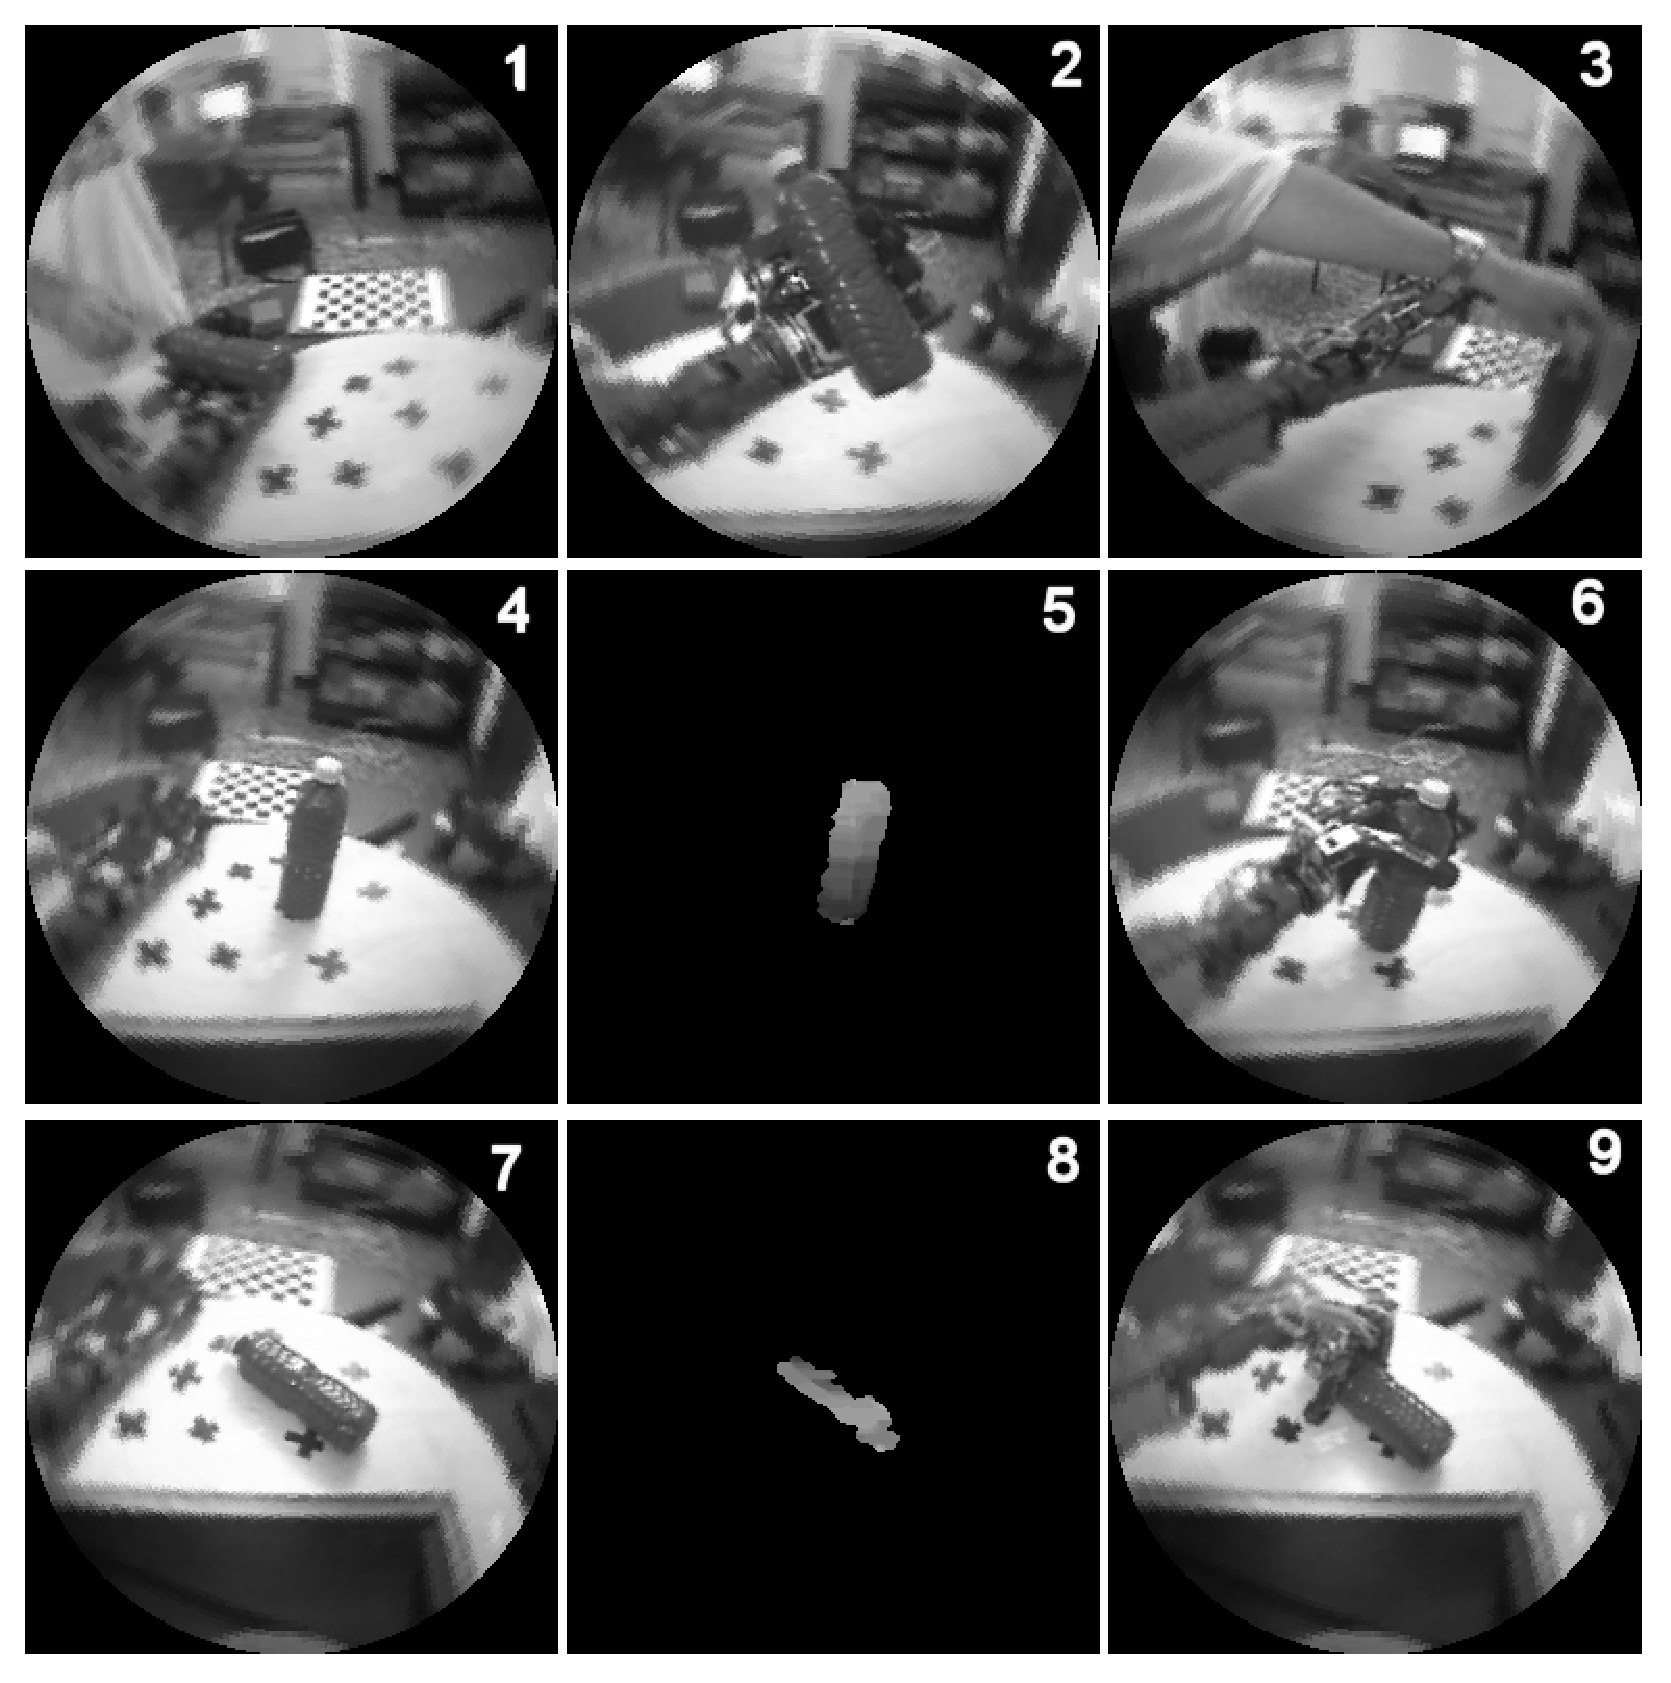
\includegraphics[width=3in]{experimental}
\caption{The execution of a grasping experiment.}
\label{fig-experiment}
\end{figure}

\section{Discussion}
Explain why someone should cite us.


\section*{Acknowledgements}

Funds for this project were provided by DARPA as
part of the ``Natural Tasking of Robots Based on Human Interaction
Cues'' project under contract number DABT 63-00-C-10102, and by the
Nippon Telegraph and Telephone Corporation as part of the NTT/MIT
Collaboration Agreement.



%  bibliography goes here
\bibliographystyle{./sty/IEEEtran}
\bibliography{main}

\end{document}
